\begin{figure}
\centering

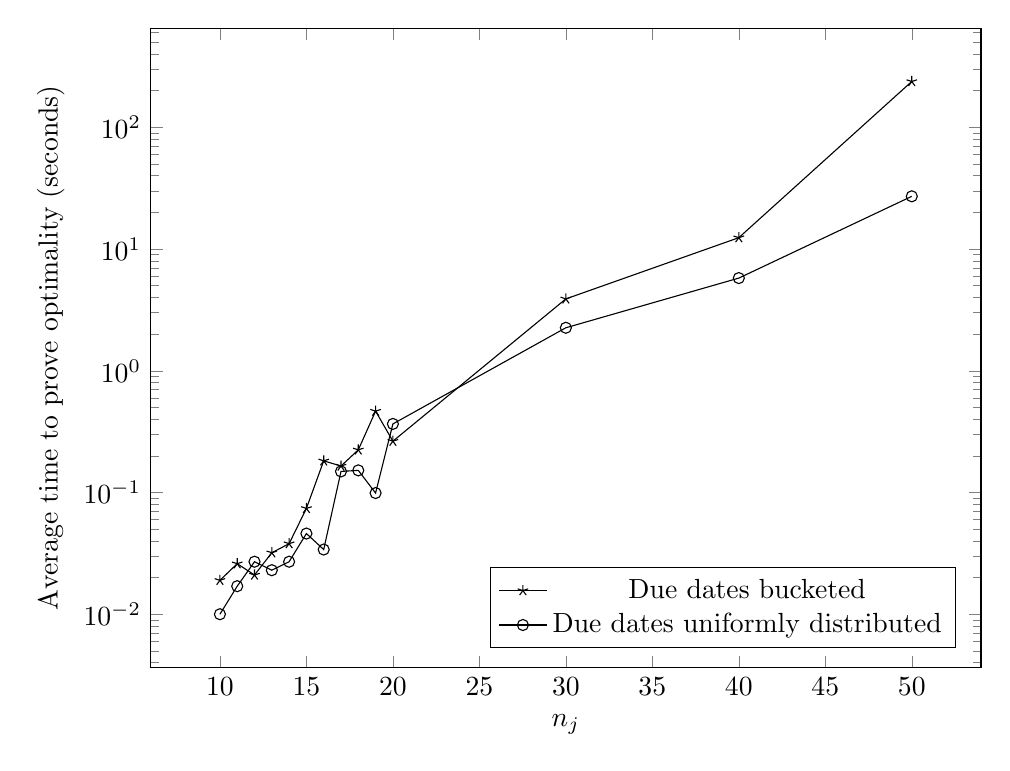
\begin{tikzpicture}
  \begin{semilogyaxis}[xlabel=$n_j$, ylabel=Average time to prove optimality (seconds), width=\textwidth,
  height=0.8\textwidth,legend pos=south east]
    \addplot[color=black, mark=star] coordinates {
(10, 0.019)
(11, 0.026)
(12, 0.021)
(13, 0.032)
(14, 0.038)
(15, 0.074)
(16, 0.182)
(17, 0.165)
(18, 0.224)
(19, 0.466)
(20, 0.264)
(30, 3.895)
(40, 12.403)
(50, 238)
};
  \addlegendentry{Due dates bucketed}
  \addplot[color=black, mark=o] coordinates {
(10, 0.01)
(11, 0.017)
(12, 0.027)
(13, 0.023)
(14, 0.027)
(15, 0.046)
(16, 0.034)
(17, 0.149)
(18, 0.152)
(19, 0.099)
(20, 0.366)
(30, 2.256)
(40, 5.775)
(50, 27.115)
};
  \addlegendentry{Due dates uniformly distributed}
  \end{semilogyaxis}
\end{tikzpicture}

\caption{Comparison of time to prove optimality required by the move-based MIP
model depending on the distribution of due dates.}
\label{fig:uniformddtimecor}
\end{figure}

